%% CoverageFlow equity research note template (cover, body, controls page).
%% Filled by coverageflow/render_note_tex.py from a report_doc dict.
%% Prose: XCharter 10pt, ragged-right, hyphenation on.  Data: Source Sans Pro.
\documentclass[10pt,a4paper]{article}
\usepackage[a4paper,top=24mm,bottom=27mm,left=18mm,right=18mm,
            headheight=12pt,headsep=7mm,footskip=9mm]{geometry}
\usepackage[T1]{fontenc}
\usepackage[utf8]{inputenc}
\usepackage{XCharter}
\usepackage[lining,tabular]{sourcesanspro}
\usepackage{xcolor}
\usepackage{fancyhdr}
\usepackage{ragged2e}
\usepackage{microtype}
\usepackage{enumitem}
\usepackage{eso-pic}
\usepackage{tikz}
\usepackage{etoolbox}
\usepackage{colortbl,booktabs}
\usepackage{multicol,tabularx,needspace,graphicx}
\setlength{\multicolsep}{3pt plus 1pt}\setlength{\columnsep}{7mm}\setlength{\columnseprule}{0.4pt}\def\columnseprulecolor{\color{hair}}

\definecolor{accent}{HTML}{1A8A4D}
\definecolor{ink}{HTML}{1C2733}
\definecolor{mute}{HTML}{51606F}
\definecolor{hair}{HTML}{CFD8DF}
\color{ink}

\newif\ifdraft
\draftfalse

\setlength{\parindent}{0pt}
\setlength{\parskip}{0pt}
\setlength{\emergencystretch}{1.5em}\hfuzz=0.5pt
\pretolerance=-1 \tolerance=1200
\hyphenpenalty=50 \exhyphenpenalty=50
\renewcommand{\arraystretch}{1.0}

%% running header / footer
\pagestyle{fancy}\fancyhf{}
\renewcommand{\headrulewidth}{0.4pt}
\renewcommand{\footrulewidth}{0pt}
\let\origheadrule\headrule
\renewcommand{\headrule}{\color{hair}\origheadrule}
\fancyhead[L]{\sffamily\fontsize{7.5}{9}\selectfont\color{mute}CoverageFlow Research  |  Equity Research  |  12 Nov 2026}
\fancyhead[R]{\sffamily\fontsize{8}{9}\selectfont\bfseries\color{accent}AMD}
\fancyfoot[L]{\sffamily\fontsize{7}{8.5}\selectfont\color{mute}Published with exceptions  ·  v1-cand-aa8  ·  information cutoff 4 Nov 2026}
\fancyfoot[R]{\sffamily\fontsize{7}{8.5}\selectfont\color{mute}\thepage\,/\,\pageref{LastPage}}
\fancyfoot[C]{}

%% draft watermark (light, diagonal, foreground: sits above the figure)
\ifdraft
\AddToShipoutPictureFG{%
  \AtPageCenter{
\begin{tikzpicture}[overlay]
    \node[opacity=0.07,text=black,rotate=54,inner sep=0pt] at (0,0)
      {\fontsize{150}{150}\selectfont\sffamily\bfseries DRAFT};
  \end{tikzpicture}}}
\fi

%% small helpers
\newcommand{\hrl}[3]{\par\nointerlineskip\vspace{#1}\noindent{\color{#2}\rule{\linewidth}{#3}}\par\nointerlineskip}
\newcommand{\sech}[1]{\par\vspace{10pt}\noindent{\sffamily\fontsize{7.5}{9}\selectfont\bfseries\color{accent}\textls[90]{\MakeUppercase{#1}}}\hrl{2pt}{accent}{0.6pt}\vspace{4pt}}
\renewcommand{\cite}[1]{\textsuperscript{\sffamily\color{accent}\fontsize{6.2}{6}\selectfont #1}}
\newcommand{\kv}[3]{{\sffamily\noindent{\fontsize{8}{10}\selectfont\color{mute}#1}\hfill{\fontsize{8.5}{10}\selectfont\bfseries#2}\par
  \ifblank{#3}{}{\noindent{\fontsize{6.5}{8}\selectfont\color{mute}\hfill#3}\par}}%
  \hrl{3pt}{hair}{0.3pt}\vspace{3pt}}
\newcommand{\sectitle}[1]{\par\Needspace{40mm}\vspace{9pt}\noindent{\sffamily\fontsize{12}{14}\selectfont\bfseries\color{ink}#1}\hrl{3pt}{accent}{0.6pt}\vspace{2pt}\fontsize{10}{13}\selectfont\setlength{\parskip}{4pt}\RaggedRight}
\newcommand{\figtitle}[1]{\noindent{\sffamily\fontsize{7.5}{9}\selectfont\bfseries\color{accent}#1\par}\vspace{2pt}}

\begin{document}
\thispagestyle{fancy}
\newlength{\sidew}\setlength{\sidew}{60mm}
\newlength{\gapw}\setlength{\gapw}{5.5mm}
\newlength{\mainw}\setlength{\mainw}{\dimexpr\textwidth-\sidew-2\gapw-0.4pt\relax}
\newlength{\colh}\setlength{\colh}{229mm}

\noindent
\begin{minipage}[t][\colh][t]{\mainw}
\RaggedRight
%% kicker, headline, byline
{\sffamily\fontsize{8}{10}\selectfont\bfseries\color{accent}\textls[100]{\MakeUppercase{AMD · Q3 FY2026 update}}}\par
\vspace{3pt}
{\sffamily\fontsize{18.5}{21.5}\selectfont\bfseries\color{ink}Data Center carries the quarter; DCF value is 90\% below the price\par}
\vspace{5pt}
{\sffamily\fontsize{7.5}{9.5}\selectfont\color{mute}CoverageFlow (automated coverage) · Published with exceptions by Gaetano Marco Chiantia, 12 Nov 2026\par}
\hrl{3pt}{hair}{0.4pt}

%% key points
\vspace{7pt}
\begin{itemize}[leftmargin=10pt,labelwidth=6pt,labelsep=4pt,itemsep=3pt,parsep=0pt,topsep=0pt,
  label={\raisebox{0.25ex}{\rule{3.2pt}{3.2pt}}}]
\item {\sffamily\fontsize{9}{11.5}\selectfont\bfseries\color{accent}Revenue\ }{\fontsize{10}{12.6}\selectfont USD~13,377mm in Q3 FY2026, +44.7\% y/y (prior-year quarter USD~9,246mm).}
\item {\sffamily\fontsize{9}{11.5}\selectfont\bfseries\color{accent}Margins\ }{\fontsize{10}{12.6}\selectfont Gross margin 53.9\% versus 51.7\% a year earlier; operating income USD~2,832mm (+123.0\% y/y), operating margin 21.2\%.}
\item {\sffamily\fontsize{9}{11.5}\selectfont\bfseries\color{accent}Earnings\ }{\fontsize{10}{12.6}\selectfont Diluted EPS USD~1.46 versus USD~0.75 in the prior-year quarter.}
\item {\sffamily\fontsize{9}{11.5}\selectfont\bfseries\color{accent}Segments\ }{\fontsize{10}{12.6}\selectfont Data Center revenue USD~8,546mm, +96.9\% y/y, 63.9\% of group; Client and Gaming \textminus{}8.1\% y/y.}
\end{itemize}

%% summary
\sech{Summary}
\fontsize{10}{13}\selectfont
AMD delivered a strong quarter, with revenue of USD~13,377mm, up 44.7\% year over year, and operating income of USD~2,832mm, up 123.0\%\cite{1--4}. Gross margin reached 53.9\%, compared with 51.7\% a year earlier, while diluted EPS increased to USD~1.46 from USD~0.75\cite{5, 6}. Data Center led the advance; Client and Gaming revenue and operating income declined year over year\cite{7--9}. Our thesis is more dependent on Data Center growth, while the quarter’s increase in inventory and accounts receivable raises execution and cash conversion questions\cite{10, 11}. The Gordon DCF indicates a target of USD~47.79 per share and a Sell rating; terminal methods diverge materially, so the output warrants caution\cite{12--14}.

%% figure
\vspace{9pt}\figtitle{Exhibit 1: Revenue by segment, Q3 FY2026 vs Q3 FY2025 (USD~mm)}\noindent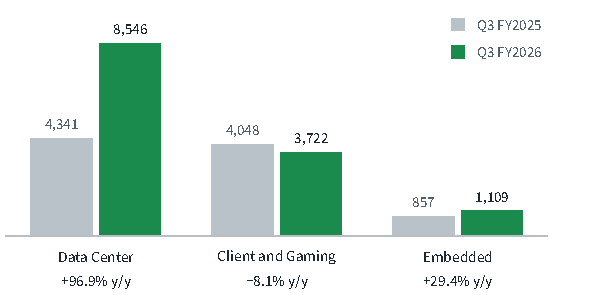
\includegraphics[width=\linewidth]{amd-fy2026q3r3-20261104-v1-cand-aa8-dossier-fig/segments.pdf}\par\vspace{1pt}{\RaggedRight\sffamily\fontsize{6.3}{7.6}\selectfont\color{mute}Source: company filings (Form 10-Q), CoverageFlow model engine.\par}

%% sources (grouped)
\vspace{2pt}
{\RaggedRight\sffamily\fontsize{6.6}{8.2}\selectfont\color{mute}\textbf{Sources.} \textbf{1, 2, 6, 10, 11}\,AMD Form 10-Q, period ended 26 Sep 2026; \textbf{3--5, 7--9}\,CoverageFlow model engine; \textbf{12--14}\,CoverageFlow valuation engine.\par}

\vfill
%% status line (hairline box, unfilled)
{\color{hair}\fboxrule 0.4pt\fboxsep 5pt\fbox{{\color{ink}\parbox{\dimexpr\linewidth-10pt-0.8pt\relax}{\RaggedRight\sffamily\fontsize{7.8}{9.8}\selectfont \textbf{Published with exceptions}: 1 open finding, \textbf{fnd-0007} (major): The note cites values that do not equal the cited ledger entries.}}}}
\end{minipage}%
\hspace{\gapw}%
{\color{hair}\vrule width 0.4pt height 9pt depth \dimexpr\colh-9pt\relax}%
\hspace{\gapw}%
\begin{minipage}[t][\colh][t]{\sidew}
\RaggedRight
{\sffamily\fontsize{7.5}{9}\selectfont\bfseries\color{accent}\textls[90]{RATING}}\par
{\sffamily\fontsize{25}{27}\selectfont\bfseries\color{ink}Sell}\par
\vspace{2pt}{\color{accent}\rule{\linewidth}{0.6pt}}\par\vspace{3pt}
\kv{Price target}{USD~47.79}{Gordon DCF; terminal methods disagree}
\kv{Price}{USD~488.78}{close, 4 Nov 2026}
\kv{Implied return}{\textminus{}90.2\%}{}
\sech{Key data}
\kv{Market cap}{USD~811,864mm}{computed: price \texttimes{} diluted shares}
\kv{Net cash}{USD~8,697mm}{Q3 FY2026}
\kv{Diluted shares}{1,661mm}{Q3 FY2026}
\kv{WACC}{10.0\%}{}
\kv{Terminal growth}{2.5\%}{}
\sech{DCF value per share}
\kv{Gordon growth}{USD~47.79}{target basis; g = 2.5\%}
\kv{Exit multiple}{USD~92.71}{21.5x terminal EBITDA}
\sech{Financial summary}
{\sffamily\fontsize{6.5}{8}\selectfont\color{mute}USD mm unless stated; EPS in USD; fiscal year\par}\vspace{2pt}
{\sffamily\fontsize{7}{9}\selectfont\setlength{\tabcolsep}{0pt}\renewcommand{\arraystretch}{1.28}
\begin{tabular*}{\linewidth}{@{}l@{\extracolsep{\fill}}r@{\extracolsep{\fill}}r@{\extracolsep{\fill}}r@{\extracolsep{\fill}}r@{\extracolsep{\fill}}r@{}}
 & \textbf{FY24A} & \textbf{FY25A} & \textbf{FY26E} & \textbf{FY27E} & \textbf{FY28E}\\\arrayrulecolor{accent}\specialrule{0.6pt}{0pt}{0pt}
Revenue & 25,785 & 34,639 & 41,798 & 49,216 & 56,512\\\arrayrulecolor{hair}\specialrule{0.3pt}{0pt}{0pt}
Growth y/y & 13.7\% & 34.3\% & 20.7\% & 17.7\% & 14.8\%\\\arrayrulecolor{hair}\specialrule{0.3pt}{0pt}{0pt}
EBITDA margin & 10.0\% & 12.8\% & 12.8\% & 12.8\% & 12.8\%\\\arrayrulecolor{hair}\specialrule{0.3pt}{0pt}{0pt}
Diluted EPS & 1.00 & 2.65 & n.a. & n.a. & n.a.\\\arrayrulecolor{hair}\specialrule{0.3pt}{0pt}{0pt}
Free cash flow & 2,405 & 6,697\textsuperscript{\textdagger} & 3,205 & 3,774 & 4,334\\\arrayrulecolor{hair}\specialrule{0.3pt}{0pt}{0pt}
\end{tabular*}}
\par\vspace{3pt}
{\sffamily\fontsize{6.3}{7.6}\selectfont\color{mute}A = reported, E = CoverageFlow DCF base case. Forecast margins held at the base-year level.\par}
{\sffamily\fontsize{6.3}{7.6}\selectfont\color{mute}EPS is not forecast by the model; forecast FCF is unlevered.\par}
{\sffamily\fontsize{6.3}{7.6}\selectfont\color{mute}\textsuperscript{\textdagger} Figure is quoted in open finding fnd-0007.\par}
\end{minipage}

\vspace{\fill}
{\RaggedRight\sffamily\fontsize{6.3}{7.8}\selectfont\color{mute}Generated by CoverageFlow from SEC filings and market data; information cutoff 4 Nov 2026. Automated analysis for a course project; not investment advice.\par}

\clearpage
\sectitle{Results}
\begin{multicols}{2}
Quarterly revenue rose to USD~13,377mm from USD~9,246mm in the prior-year quarter\cite{1}. Gross profit increased to USD~7,210mm from USD~4,780mm, and gross margin expanded to 53.9\% from 51.7\%\cite{1, 5, 15}. Operating income grew to USD~2,832mm, with operating margin rising to 21.2\% from 13.7\%\cite{2, 16}. The improvement reflects revenue growth and higher gross profit, partly offset by higher operating expenses, which increased to USD~4,378mm from USD~3,510mm\cite{15, 17}.

Net income was USD~2,428mm versus USD~1,243mm, and diluted EPS was USD~1.46 versus USD~0.75\cite{6, 18}. Other income (expense), net was an expense of USD~902mm, compared with income of USD~82mm in the prior-year quarter; interest expense was USD~62mm versus USD~37mm\cite{19, 20}. The non-operating line partly offset the improvement in operating income. For the nine months ended in Q3, revenue was USD~35,166mm versus USD~24,369mm, while operating income was USD~6,298mm versus USD~1,942mm\cite{1, 2}.

Operating cash flow for the nine-month period was USD~6,523mm, up from USD~5,109mm\cite{21}. Cash and cash equivalents at quarter end were USD~7,404mm, and short-term investments were USD~8,372mm\cite{21--23}. The company reported USD~7,079mm of long-term debt and no current portion of long-term debt; the model’s net-debt measure was negative USD~8,697mm, indicating net cash\cite{24--26}.
\end{multicols}
\par\vspace{9pt}\noindent\begin{minipage}[t]{\linewidth}
\sffamily\fontsize{7.5}{9.5}\selectfont
{\RaggedRight\bfseries\color{accent}Exhibit 2\hspace{0.7em}\color{ink}Income statement summary, Q3 FY2026 vs Q3 FY2025\par}
{\color{mute}\fontsize{6.5}{8}\selectfont USD~mm except per share\par}\hrl{2pt}{accent}{0.6pt}\vspace{1pt}
{\setlength{\tabcolsep}{1.5pt}\renewcommand{\arraystretch}{1.2}\RaggedRight
\begin{tabular*}{\linewidth}{@{}>{\RaggedRight}p{60mm}@{\extracolsep{\fill}}r@{\extracolsep{\fill}}r@{\extracolsep{\fill}}r@{\extracolsep{\fill}}r@{\extracolsep{\fill}}r@{\extracolsep{\fill}}r@{}}
 & \textbf{Q3 FY2026} & \textbf{Q3 FY2025} & \textbf{y/y} & \textbf{9M FY2026} & \textbf{9M FY2025} & \textbf{y/y}\\\arrayrulecolor{accent}\specialrule{0.6pt}{0pt}{0pt}
Revenue & 13,377 & 9,246 & +44.7\% & 35,166 & 24,369 & +44.3\%\\\arrayrulecolor{hair}\specialrule{0.3pt}{0pt}{0pt}
Gross profit & 7,210 & 4,780 & +50.8\% & 18,829 & 11,575 & +62.7\%\\\arrayrulecolor{hair}\specialrule{0.3pt}{0pt}{0pt}
\textcolor{mute}{Gross margin} & \textcolor{mute}{53.9\%} & \textcolor{mute}{51.7\%} & \textcolor{mute}{+2.2 pp} & \textcolor{mute}{53.5\%} & \textcolor{mute}{47.5\%} & \textcolor{mute}{+6.0 pp}\\\arrayrulecolor{hair}\specialrule{0.3pt}{0pt}{0pt}
Operating expenses & 4,378 & 3,510 & +24.7\% & 12,531 & 9,633 & +30.1\%\\\arrayrulecolor{hair}\specialrule{0.3pt}{0pt}{0pt}
Operating income & 2,832 & 1,270 & +123.0\% & 6,298 & 1,942 & +224.3\%\\\arrayrulecolor{hair}\specialrule{0.3pt}{0pt}{0pt}
\textcolor{mute}{Operating margin} & \textcolor{mute}{21.2\%} & \textcolor{mute}{13.7\%} & \textcolor{mute}{+7.4 pp} & \textcolor{mute}{17.9\%} & \textcolor{mute}{8.0\%} & \textcolor{mute}{+9.9 pp}\\\arrayrulecolor{hair}\specialrule{0.3pt}{0pt}{0pt}
Net income & 2,428 & 1,243 & +95.3\% & 6,108 & 2,824 & +116.3\%\\\arrayrulecolor{hair}\specialrule{0.3pt}{0pt}{0pt}
Diluted EPS (USD) & 1.46 & 0.75 & +94.7\% & 3.69 & 1.73 & +113.3\%\\\arrayrulecolor{hair}\specialrule{0.3pt}{0pt}{0pt}
\end{tabular*}}
\par\vspace{2pt}{\RaggedRight\color{mute}\fontsize{6.4}{7.8}\selectfont
Source: company filings (SEC), CoverageFlow model engine (model\_engine@1.0).\par}
\end{minipage}\par
\sectitle{Segment detail}
\begin{multicols}{2}
Data Center revenue increased to USD~8,546mm from USD~4,341mm, and segment operating income rose to USD~2,882mm from USD~1,074mm\cite{7, 27}. The operating margin increased to 33.7\% from 24.7\%\cite{7, 27, 28}. Data Center generated the clear majority of quarterly revenue and operating profit growth. Nine-month revenue reached USD~21,039mm, compared with USD~11,255mm, while operating income was USD~6,584mm versus USD~1,851mm\cite{7, 27}.

Client and Gaming revenue declined to USD~3,722mm from USD~4,048mm\cite{8}. Segment operating income fell to USD~573mm from USD~867mm, and operating margin narrowed to 15.4\% from 21.4\%\cite{8, 9, 29}. The nine-month comparison was firmer: revenue increased to USD~11,168mm from USD~10,610mm, though operating income was USD~1,730mm versus USD~2,130mm\cite{8, 9}.

Embedded revenue advanced to USD~1,109mm from USD~857mm\cite{30}. Operating income was USD~453mm versus USD~283mm, with margin of 40.8\% compared with 33.0\%\cite{30--32}. Nine-month revenue grew to USD~2,959mm from USD~2,504mm, and operating income rose to USD~1,177mm from USD~886mm\cite{30, 31}. All Other recorded an operating loss of USD~1,076mm, wider than the USD~954mm loss in the prior-year quarter\cite{33}.
\end{multicols}
\par\vspace{9pt}\noindent\begin{minipage}[t]{\linewidth}
\sffamily\fontsize{7.5}{9.5}\selectfont
{\RaggedRight\bfseries\color{accent}Exhibit 3\hspace{0.7em}\color{ink}Segment results, Q3 FY2026\par}
{\color{mute}\fontsize{6.5}{8}\selectfont USD~mm\par}\hrl{2pt}{accent}{0.6pt}\vspace{1pt}
{\setlength{\tabcolsep}{1.5pt}\renewcommand{\arraystretch}{1.2}\RaggedRight
\begin{tabular*}{\linewidth}{@{}>{\RaggedRight}p{55mm}@{\extracolsep{\fill}}r@{\extracolsep{\fill}}r@{\extracolsep{\fill}}r@{\extracolsep{\fill}}r@{\extracolsep{\fill}}r@{\extracolsep{\fill}}r@{\extracolsep{\fill}}r@{}}
 & \begin{tabular}[b]{@{}r@{}}\textbf{Revenue}\\\textbf{Q3 FY2026}\end{tabular} & \textbf{y/y} & \begin{tabular}[b]{@{}r@{}}\textbf{\% of}\\\textbf{group}\end{tabular} & \begin{tabular}[b]{@{}r@{}}\textbf{Op.}\\\textbf{income}\end{tabular} & \begin{tabular}[b]{@{}r@{}}\textbf{Op.}\\\textbf{margin}\end{tabular} & \begin{tabular}[b]{@{}r@{}}\textbf{Revenue}\\\textbf{9M FY2026}\end{tabular} & \begin{tabular}[b]{@{}r@{}}\textbf{Op. income}\\\textbf{9M FY2026}\end{tabular}\\\arrayrulecolor{accent}\specialrule{0.6pt}{0pt}{0pt}
Data Center & 8,546 & +96.9\% & 63.9\% & 2,882 & 33.7\% & 21,039 & 6,584\\\arrayrulecolor{hair}\specialrule{0.3pt}{0pt}{0pt}
Client and Gaming & 3,722 & \textminus{}8.1\% & 27.8\% & 573 & 15.4\% & 11,168 & 1,730\\\arrayrulecolor{hair}\specialrule{0.3pt}{0pt}{0pt}
Embedded & 1,109 & +29.4\% & 8.3\% & 453 & 40.8\% & 2,959 & 1,177\\\arrayrulecolor{hair}\specialrule{0.3pt}{0pt}{0pt}
All other & n.a. & n.a. & n.a. & \textminus{}1,076 & n.a. & n.a. & \textminus{}3,193\\\arrayrulecolor{hair}\specialrule{0.3pt}{0pt}{0pt}
\textbf{Group} & \textbf{13,377} & \textbf{+44.7\%} & \textbf{100.0\%} & \textbf{2,832} & \textbf{21.2\%} & \textbf{35,166} & \textbf{6,298}\\\arrayrulecolor{hair}\specialrule{0.3pt}{0pt}{0pt}
\end{tabular*}}
\par\vspace{2pt}{\RaggedRight\color{mute}\fontsize{6.4}{7.8}\selectfont
Source: company filings (SEC, segment note), CoverageFlow model engine (model\_engine@1.0).\par}
\end{minipage}\par
\sectitle{Outlook}
\begin{multicols}{2}
Our forecast path assumes that Data Center remains the principal growth contributor, with growth moderating over time. That direction is consistent with the step-up in Data Center quarterly and nine-month revenue, while the prior-year comparison is increasingly demanding\cite{7}. The path assumes a more measured contribution from Client and Gaming after its quarterly revenue decline and lower segment operating income\cite{8, 9}. Embedded is modeled as a gradual recovery, supported by the quarterly and nine-month increases in revenue and operating income, while recognizing its history of lower annual revenue\cite{30, 31}.

The valuation uses FY2025 as its base because the supplied nine-month cash-flow history does not provide the capital-expenditure inputs needed to construct a trailing twelve-month base. The historical base was revenue of USD~34,639mm, EBITDA of USD~4,444mm, and free cash flow of USD~6,697mm\cite{34--37}. Those reported cash flows support the model’s starting point, but they do not remove the uncertainty around sustained growth, margins, or investment needs.
\end{multicols}
\sectitle{Valuation}
\begin{multicols}{2}
The DCF uses a 10.0\% WACC and 2.5\% terminal growth\cite{13, 38, 39}. The Gordon method produces equity value of USD~79,383mm and USD~47.79 per diluted share\cite{12, 40}. The exit-multiple method, using 21.5x EBITDA, produces equity value of USD~153,989mm and USD~92.71 per diluted share\cite{14, 41--43}. The terminal values are USD~79,354mm under Gordon and USD~190,106mm under the exit-multiple method; the model flags this gap as outside its tolerance\cite{13, 14}. We therefore use the Gordon output as the target basis, with the divergence showing how sensitive the DCF is to terminal assumptions.

The relative valuation applies peer medians to AMD’s FY2025 metrics and yields an indicated value of USD~145.52 per share\cite{44}. The model’s DCF and relative-valuation cross-check delta is negative 20.0\%, within the stated mandate tolerance, although the terminal methods remain far apart\cite{45}. The peer-derived EV/EBITDA range is broad, from 18.74x to 153.83x, which limits the precision of a single multiple-based conclusion\cite{44}. We retain the Gordon target of USD~47.79 per share and Sell rating\cite{12}.
\end{multicols}
\par\vspace{9pt}\noindent\begin{minipage}[t]{\linewidth}
\sffamily\fontsize{7.5}{9.5}\selectfont
{\RaggedRight\bfseries\color{accent}Exhibit 4\hspace{0.7em}\color{ink}DCF summary\par}
{\color{mute}\fontsize{6.5}{8}\selectfont USD~mm\par}\hrl{2pt}{accent}{0.6pt}\vspace{1pt}
{\setlength{\tabcolsep}{1.5pt}\renewcommand{\arraystretch}{1.2}\RaggedRight
\begin{tabular*}{\linewidth}{@{}>{\RaggedRight}p{60mm}@{\extracolsep{\fill}}r@{\extracolsep{\fill}}r@{\extracolsep{\fill}}r@{\extracolsep{\fill}}r@{\extracolsep{\fill}}r@{\extracolsep{\fill}}r@{}}
 & \textbf{FY2025A} & \textbf{FY2026E} & \textbf{FY2027E} & \textbf{FY2028E} & \textbf{FY2029E} & \textbf{FY2030E}\\\arrayrulecolor{accent}\specialrule{0.6pt}{0pt}{0pt}
Revenue & 34,639 & 41,798 & 49,216 & 56,512 & 63,239 & 68,921\\\arrayrulecolor{hair}\specialrule{0.3pt}{0pt}{0pt}
Growth y/y & +34.3\% & +20.7\% & +17.7\% & +14.8\% & +11.9\% & +9.0\%\\\arrayrulecolor{hair}\specialrule{0.3pt}{0pt}{0pt}
EBITDA & 4,444 & 5,362 & 6,314 & 7,250 & 8,113 & 8,842\\\arrayrulecolor{hair}\specialrule{0.3pt}{0pt}{0pt}
\textcolor{mute}{EBITDA margin} & \textcolor{mute}{12.8\%} & \textcolor{mute}{12.8\%} & \textcolor{mute}{12.8\%} & \textcolor{mute}{12.8\%} & \textcolor{mute}{12.8\%} & \textcolor{mute}{12.8\%}\\\arrayrulecolor{hair}\specialrule{0.3pt}{0pt}{0pt}
EBIT & 3,694 & 4,457 & 5,248 & 6,027 & 6,744 & 7,350\\\arrayrulecolor{hair}\specialrule{0.3pt}{0pt}{0pt}
Capital expenditure & 1,012 & 1,221 & 1,438 & 1,651 & 1,848 & 2,014\\\arrayrulecolor{hair}\specialrule{0.3pt}{0pt}{0pt}
\textbf{Free cash flow} & \textbf{6,697\textsuperscript{\textdagger}} & \textbf{3,205} & \textbf{3,774} & \textbf{4,334} & \textbf{4,849} & \textbf{5,285}\\\arrayrulecolor{hair}\specialrule{0.3pt}{0pt}{0pt}
Discount factor & n.a. & 0.9863 & 0.8967 & 0.8150 & 0.7409 & 0.6736\\\arrayrulecolor{hair}\specialrule{0.3pt}{0pt}{0pt}
\textbf{PV of free cash flow} & \textbf{n.a.} & \textbf{3,161} & \textbf{3,384} & \textbf{3,532} & \textbf{3,593} & \textbf{3,560}\\\arrayrulecolor{hair}\specialrule{0.3pt}{0pt}{0pt}
\end{tabular*}}
\par\vspace{2pt}{\RaggedRight\color{mute}\fontsize{6.4}{7.8}\selectfont
Discounting: year end at WACC 10.0\%; valuation date 2026-11-04.\par
Base year: fiscal-year fallback (trailing-twelve-month base could not be built).\par
\textsuperscript{\textdagger} Figure is quoted in open finding fnd-0007.\par
Source: CoverageFlow valuation engine (valuation\_engine@2.0), dcf.years.\par}
\end{minipage}\par
\par\vspace{9pt}\noindent\begin{minipage}[t]{0.485\linewidth}
\sffamily\fontsize{7.5}{9.5}\selectfont
{\RaggedRight\bfseries\color{accent}Exhibit 5\hspace{0.7em}\color{ink}From enterprise value to value per share\par}
{\color{mute}\fontsize{6.5}{8}\selectfont USD~mm\par}\hrl{2pt}{accent}{0.6pt}\vspace{1pt}
{\setlength{\tabcolsep}{1.5pt}\renewcommand{\arraystretch}{1.2}\RaggedRight
\begin{tabular*}{\linewidth}{@{}>{\RaggedRight}p{57mm}@{\extracolsep{\fill}}r@{\extracolsep{\fill}}r@{}}
 & \begin{tabular}[b]{@{}r@{}}\textbf{Gordon}\\\textbf{growth}\end{tabular} & \begin{tabular}[b]{@{}r@{}}\textbf{Exit}\\\textbf{multiple}\end{tabular}\\\arrayrulecolor{accent}\specialrule{0.6pt}{0pt}{0pt}
PV of free cash flow & 17,230 & 17,230\\\arrayrulecolor{hair}\specialrule{0.3pt}{0pt}{0pt}
Terminal value & 79,354 & 190,106\\\arrayrulecolor{hair}\specialrule{0.3pt}{0pt}{0pt}
PV of terminal value & 53,456 & 128,061\\\arrayrulecolor{hair}\specialrule{0.3pt}{0pt}{0pt}
\textbf{Enterprise value} & \textbf{70,686} & \textbf{145,292}\\\arrayrulecolor{hair}\specialrule{0.3pt}{0pt}{0pt}
Less: net debt (negative = net cash) & \textminus{}8,697 & \textminus{}8,697\\\arrayrulecolor{hair}\specialrule{0.3pt}{0pt}{0pt}
Less: non-controlling interests & n.a. & n.a.\\\arrayrulecolor{hair}\specialrule{0.3pt}{0pt}{0pt}
\textbf{Equity value} & \textbf{79,383} & \textbf{153,989}\\\arrayrulecolor{hair}\specialrule{0.3pt}{0pt}{0pt}
Diluted shares (mm) & 1,661 & 1,661\\\arrayrulecolor{hair}\specialrule{0.3pt}{0pt}{0pt}
\textbf{Value per share (USD)} & \textbf{47.79} & \textbf{92.71}\\\arrayrulecolor{hair}\specialrule{0.3pt}{0pt}{0pt}
\textcolor{mute}{Implied terminal EV/EBITDA} & \textcolor{mute}{9.0x} & \textcolor{mute}{21.5x}\\\arrayrulecolor{hair}\specialrule{0.3pt}{0pt}{0pt}
\textcolor{mute}{Implied terminal growth} & \textcolor{mute}{2.5\%} & \textcolor{mute}{6.7\%}\\\arrayrulecolor{hair}\specialrule{0.3pt}{0pt}{0pt}
\end{tabular*}}
\par\vspace{2pt}{\RaggedRight\color{mute}\fontsize{6.4}{7.8}\selectfont
Source: CoverageFlow valuation engine (valuation\_engine@2.0), dcf.ev / bridge / terminal.\par}
\end{minipage}\hfill\begin{minipage}[t]{0.485\linewidth}
\sffamily\fontsize{7.5}{9.5}\selectfont
{\RaggedRight\bfseries\color{accent}Exhibit 6\hspace{0.7em}\color{ink}Gordon DCF value per share by WACC and terminal growth\par}
{\color{mute}\fontsize{6.5}{8}\selectfont USD~per share\par}\hrl{2pt}{accent}{0.6pt}\vspace{1pt}
{\setlength{\tabcolsep}{1.5pt}\renewcommand{\arraystretch}{1.2}\RaggedRight
\begin{tabular*}{\linewidth}{@{}>{\RaggedRight}p{17mm}@{\extracolsep{\fill}}r@{\extracolsep{\fill}}r@{\extracolsep{\fill}}r@{\extracolsep{\fill}}r@{\extracolsep{\fill}}r@{}}
\begin{tabular}[b]{@{}r@{}}\textbf{WACC /}\\\textbf{growth}\end{tabular} & \textbf{0.5\%} & \textbf{1.5\%} & \textbf{2.5\%} & \textbf{3.5\%} & \textbf{4.5\%}\\\arrayrulecolor{accent}\specialrule{0.6pt}{0pt}{0pt}
6.0\% & 66.68 & 78.44 & 96.91 & 130.18 & 207.79\\\arrayrulecolor{hair}\specialrule{0.3pt}{0pt}{0pt}
8.0\% & 50.09 & 55.72 & 63.39 & 74.48 & 91.91\\\arrayrulecolor{hair}\specialrule{0.3pt}{0pt}{0pt}
10.0\% & 40.52 & 43.73 & \setlength{\fboxsep}{1.2pt}\setlength{\fboxrule}{0.6pt}\fcolorbox{accent}{white}{\strut 47.79} & 53.11 & 60.35\\\arrayrulecolor{hair}\specialrule{0.3pt}{0pt}{0pt}
12.0\% & 34.31 & 36.33 & 38.79 & 41.82 & 45.66\\\arrayrulecolor{hair}\specialrule{0.3pt}{0pt}{0pt}
14.0\% & 29.95 & 31.33 & 32.94 & 34.85 & 37.17\\\arrayrulecolor{hair}\specialrule{0.3pt}{0pt}{0pt}
\end{tabular*}}
\par\vspace{2pt}{\RaggedRight\color{mute}\fontsize{6.4}{7.8}\selectfont
Rows: WACC; columns: terminal growth. Boxed cell is the base case.\par
Source: CoverageFlow valuation engine (valuation\_engine@2.0), sensitivity.grid.\par}
\end{minipage}\par
\par\vspace{9pt}\noindent\begin{minipage}[t]{0.485\linewidth}
\sffamily\fontsize{7.5}{9.5}\selectfont
{\RaggedRight\bfseries\color{accent}Exhibit 7\hspace{0.7em}\color{ink}Peer multiples\par}
{\color{mute}\fontsize{6.5}{8}\selectfont as of 4 Nov 2026\par}\hrl{2pt}{accent}{0.6pt}\vspace{1pt}
{\setlength{\tabcolsep}{1.5pt}\renewcommand{\arraystretch}{1.2}\RaggedRight
\begin{tabular*}{\linewidth}{@{}>{\RaggedRight}p{27mm}@{\extracolsep{\fill}}r@{\extracolsep{\fill}}r@{\extracolsep{\fill}}r@{\extracolsep{\fill}}r@{}}
 & \textbf{EV/EBITDA} & \textbf{P/E (TTM)} & \textbf{P/S} & \begin{tabular}[b]{@{}r@{}}\textbf{Rev.}\\\textbf{growth}\end{tabular}\\\arrayrulecolor{accent}\specialrule{0.6pt}{0pt}{0pt}
INTC & 153.8x & n.a. & 5.2x & \textminus{}0.5\%\\\arrayrulecolor{hair}\specialrule{0.3pt}{0pt}{0pt}
NVDA & 24.2x & 25.2x & 16.0x & +65.5\%\\\arrayrulecolor{hair}\specialrule{0.3pt}{0pt}{0pt}
QCOM & 18.7x & 13.6x & 4.3x & \textminus{}2.6\%\\\arrayrulecolor{hair}\specialrule{0.3pt}{0pt}{0pt}
AVGO & n.a. & 41.6x & 17.9x & +23.9\%\\\arrayrulecolor{hair}\specialrule{0.3pt}{0pt}{0pt}
\textbf{Median} & \textbf{24.2x} & \textbf{n.a.} & \textbf{10.6x} & \textbf{n.a.}\\\arrayrulecolor{hair}\specialrule{0.3pt}{0pt}{0pt}
\end{tabular*}}
\par\vspace{2pt}{\RaggedRight\color{mute}\fontsize{6.4}{7.8}\selectfont
Source: SEC companyfacts and closing prices (peer block), CoverageFlow valuation engine (valuation\_engine@2.0).\par}
\end{minipage}\hfill\begin{minipage}[t]{0.485\linewidth}
\sffamily\fontsize{7.5}{9.5}\selectfont
{\RaggedRight\bfseries\color{accent}Exhibit 8\hspace{0.7em}\color{ink}Relative valuation of AMD\par}
{\color{mute}\fontsize{6.5}{8}\selectfont USD~mm; per share in USD\par}\hrl{2pt}{accent}{0.6pt}\vspace{1pt}
{\setlength{\tabcolsep}{1.5pt}\renewcommand{\arraystretch}{1.2}\RaggedRight
\begin{tabular*}{\linewidth}{@{}>{\RaggedRight}p{42mm}@{\extracolsep{\fill}}r@{\extracolsep{\fill}}r@{\extracolsep{\fill}}r@{}}
 & \begin{tabular}[b]{@{}r@{}}\textbf{AMD}\\\textbf{metric}\end{tabular} & \begin{tabular}[b]{@{}r@{}}\textbf{Peer}\\\textbf{median}\end{tabular} & \textbf{Per share}\\\arrayrulecolor{accent}\specialrule{0.6pt}{0pt}{0pt}
EV/EBITDA on FY2025 EBITDA & 4,444 & 24.2x & 69.98\\\arrayrulecolor{hair}\specialrule{0.3pt}{0pt}{0pt}
P/S on FY2025 revenue & 34,639 & 10.6x & 221.06\\\arrayrulecolor{hair}\specialrule{0.3pt}{0pt}{0pt}
\textbf{Comps-implied value (average)} & \textbf{} & \textbf{} & \textbf{145.52\textsuperscript{\textdagger}}\\\arrayrulecolor{hair}\specialrule{0.3pt}{0pt}{0pt}
\end{tabular*}}
\par\vspace{2pt}{\RaggedRight\color{mute}\fontsize{6.4}{7.8}\selectfont
Comps-implied value versus price: \textminus{}70.2\%.\par
DCF and relative valuation agree within mandate tolerance.\par
\textsuperscript{\textdagger} Figure is quoted in open finding fnd-0007.\par
Source: CoverageFlow valuation engine (valuation\_engine@2.0), comps.applied.\par}
\end{minipage}\par
\par\vspace{9pt}\noindent\begin{minipage}[t]{\linewidth}
\sffamily\fontsize{7.5}{9.5}\selectfont
{\RaggedRight\bfseries\color{accent}Exhibit 9\hspace{0.7em}\color{ink}Valuation range, USD~per share\par}
{\color{mute}\fontsize{6.5}{8}\selectfont USD~per share\par}\hrl{2pt}{accent}{0.6pt}\vspace{1pt}
\vspace{2pt}\noindent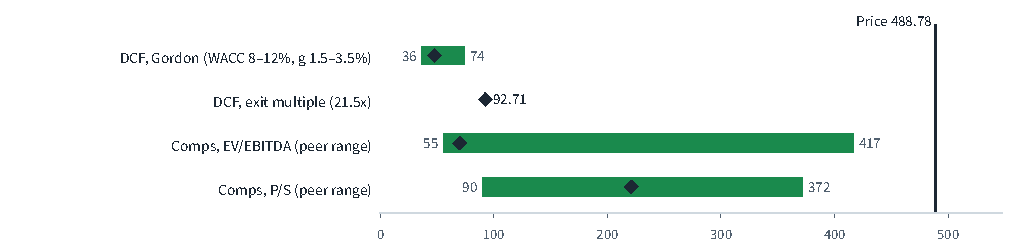
\includegraphics[width=\linewidth]{amd-fy2026q3r3-20261104-v1-cand-aa8-dossier-fig/football.pdf}
\par\vspace{2pt}{\RaggedRight\color{mute}\fontsize{6.4}{7.8}\selectfont
Bars show ranges, diamonds the point estimate (median multiple, base-case DCF); the vertical line is the share price.\par
Source: CoverageFlow valuation engine (valuation\_engine@2.0), dcf, sensitivity, comps.\par}
\end{minipage}\par
\sectitle{Risks}
\begin{multicols}{2}
The principal operating risk is that growth remains concentrated in Data Center while other segments contribute less. Data Center represented 63.9\% of quarterly revenue; Client and Gaming revenue declined, and All Other’s operating loss widened\cite{8, 33, 46}. A slowdown in the largest segment would therefore weigh heavily on consolidated results.

Working capital is another watch point. Inventory rose to USD~11,463mm from USD~7,920mm at FY2025, while accounts receivable increased to USD~9,209mm from USD~6,315mm\cite{10, 11}. If shipments or customer collections weaken, these balances could constrain cash conversion. Finally, the terminal-value spread between valuation methods makes the target sensitive to assumptions about long-run growth and exit value; the Gordon DCF is substantially below the exit-multiple result\cite{13, 14}.
\end{multicols}
\clearpage
\sectitle{Sources and controls}
\par\vspace{7pt}{\sffamily\fontsize{7.5}{9}\selectfont\bfseries\color{accent}\textls[90]{INPUT DOCUMENTS}\par}\vspace{2pt}
{\setlength{\tabcolsep}{2pt}\renewcommand{\arraystretch}{1.2}\sffamily\fontsize{7}{8.6}\selectfont
\begin{tabularx}{\linewidth}{@{}>{\RaggedRight\arraybackslash}X>{\RaggedRight\arraybackslash}p{14mm}>{\RaggedRight\arraybackslash}p{24mm}>{\RaggedRight\arraybackslash}p{22mm}>{\RaggedRight\arraybackslash}p{30mm}@{}}
\textbf{Document} & \textbf{Form} & \textbf{Period ended} & \textbf{Filed} & \textbf{SHA-256 (first 12)}\\\arrayrulecolor{accent}\specialrule{0.6pt}{0pt}{0pt}
amd-10k-fy2024 & 10-K & 28 Dec 2024 & 5 Feb 2025 & 9f1e660458aa\\\arrayrulecolor{hair}\specialrule{0.3pt}{0pt}{0pt}
amd-10k-fy2025 & 10-K & 27 Dec 2025 & 4 Feb 2026 & 24724a71abca\\\arrayrulecolor{hair}\specialrule{0.3pt}{0pt}{0pt}
amd-10q-2025q1 & 10-Q & 29 Mar 2025 & 7 May 2025 & 38837430579f\\\arrayrulecolor{hair}\specialrule{0.3pt}{0pt}{0pt}
amd-10q-2025q2 & 10-Q & 28 Jun 2025 & 6 Aug 2025 & 95bda811f43e\\\arrayrulecolor{hair}\specialrule{0.3pt}{0pt}{0pt}
amd-10q-2025q3 & 10-Q & 27 Sep 2025 & 5 Nov 2025 & c470cdf079a6\\\arrayrulecolor{hair}\specialrule{0.3pt}{0pt}{0pt}
amd-10q-2026q1 & 10-Q & 28 Mar 2026 & 6 May 2026 & 7e04ff77ce5d\\\arrayrulecolor{hair}\specialrule{0.3pt}{0pt}{0pt}
amd-10q-2026q2 & 10-Q & 27 Jun 2026 & 5 Aug 2026 & 2940323fe639\\\arrayrulecolor{hair}\specialrule{0.3pt}{0pt}{0pt}
amd-10q-2026q3 & 10-Q & 26 Sep 2026 & 4 Nov 2026 & 11ee28589c28\\\arrayrulecolor{hair}\specialrule{0.3pt}{0pt}{0pt}
amd-8k-2025-10-27 & 8-K & 27 Oct 2025 & 27 Oct 2025 & 548e7022ca42\\\arrayrulecolor{hair}\specialrule{0.3pt}{0pt}{0pt}
amd-8k-2026-11-03 & 8-K & 3 Nov 2026 & 3 Nov 2026 & fb8c8664131a\\\arrayrulecolor{hair}\specialrule{0.3pt}{0pt}{0pt}
\end{tabularx}}
\par\vspace{7pt}{\sffamily\fontsize{7.5}{9}\selectfont\bfseries\color{accent}\textls[90]{EVIDENCE REFERENCES}\par}\vspace{2pt}
{\setlength{\tabcolsep}{2pt}\renewcommand{\arraystretch}{1.2}\sffamily\fontsize{7}{8.6}\selectfont
\begin{tabularx}{\linewidth}{@{}>{\RaggedRight\arraybackslash}p{14mm}>{\RaggedRight\arraybackslash}p{52mm}>{\RaggedRight\arraybackslash}p{40mm}>{\RaggedRight\arraybackslash}X@{}}
\textbf{Ref.} & \textbf{Source} & \textbf{Statement} & \textbf{Items cited}\\\arrayrulecolor{accent}\specialrule{0.6pt}{0pt}{0pt}
1, 2, 6, 15, 17--20 & AMD Form 10-Q, period ended 26 Sep 2026 & Condensed Consolidated Statements of Operations & Net revenue; Operating income; Diluted earnings per share; Gross profit; Total operating expenses; Net income; Other income (expense), net; Interest expense\\\arrayrulecolor{hair}\specialrule{0.3pt}{0pt}{0pt}
10, 11, 22--25 & AMD Form 10-Q, period ended 26 Sep 2026 & Condensed Consolidated Balance Sheets & Inventories; Accounts receivable, net; Cash and cash equivalents; Short-term investments; Long-term debt, net; Current portion of long-term debt, net\\\arrayrulecolor{hair}\specialrule{0.3pt}{0pt}{0pt}
21 & AMD Form 10-Q, period ended 26 Sep 2026 & Condensed Consolidated Statements of Cash Flows & Net cash provided by operating activities\\\arrayrulecolor{hair}\specialrule{0.3pt}{0pt}{0pt}
33 & AMD Form 10-Q, period ended 26 Sep 2026 & NOTE 4 -- Segment Reporting & All other\\\arrayrulecolor{hair}\specialrule{0.3pt}{0pt}{0pt}
36 & AMD Form 10-K, period ended 27 Dec 2025 & Consolidated Statements of Cash Flows & Purchases of property and equipment\\\arrayrulecolor{hair}\specialrule{0.3pt}{0pt}{0pt}
3--5, 7--9, 16, 26--32, 46 & CoverageFlow model engine & Model series & derived: revenue\_yoy, operating\_income\_yoy, gross\_margin, operating\_margin, net\_debt; segments: data\_center.revenue, client\_and\_gaming.revenue, client\_and\_gaming.operating\_income, data\_center.operating\_income, data\_center.operating\_margin, client\_and\_gaming.operating\_margin, embedded.revenue, embedded.operating\_income, embedded.operating\_margin, data\_center.revenue\_share\_of\_total\\\arrayrulecolor{hair}\specialrule{0.3pt}{0pt}{0pt}
12--14, 34, 35, 37--45 & CoverageFlow valuation engine & Valuation outputs & dcf: per\_diluted\_share.gordon, terminal.gordon.terminal\_value, terminal.exit\_multiple.terminal\_value, base.revenue, base.ebitda\_margin, wacc, terminal.gordon.terminal\_growth, equity\_value.gordon, per\_diluted\_share.exit\_multiple, equity\_value.exit\_multiple; comps: applied.ev\_ebitda.own\_metric, own\_band; assumptions: exit\_multiple\_ebitda; cross\_check\_delta: cross\_check\_delta\\\arrayrulecolor{hair}\specialrule{0.3pt}{0pt}{0pt}
\end{tabularx}}
\par\vspace{7pt}{\sffamily\fontsize{7.5}{9}\selectfont\bfseries\color{accent}\textls[90]{DECISION RECORD}\par}\vspace{2pt}
{\setlength{\tabcolsep}{2pt}\renewcommand{\arraystretch}{1.2}\sffamily\fontsize{7}{8.6}\selectfont
\begin{tabularx}{\linewidth}{@{}>{\RaggedRight\arraybackslash}p{17mm}>{\RaggedRight\arraybackslash}p{44mm}>{\RaggedRight\arraybackslash}p{34mm}>{\RaggedRight\arraybackslash}p{20mm}>{\RaggedRight\arraybackslash}X@{}}
\textbf{Record} & \textbf{Decision} & \textbf{By} & \textbf{Date} & \textbf{Reasoning}\\\arrayrulecolor{accent}\specialrule{0.6pt}{0pt}{0pt}
apr-0001 & PUBLISHED\_WITH\_EXCEPTIONS & Gaetano Marco Chiantia & 12 Nov 2026 & Approved.\\\arrayrulecolor{hair}\specialrule{0.3pt}{0pt}{0pt}
\end{tabularx}}
\par\vspace{7pt}{\sffamily\fontsize{7.5}{9}\selectfont\bfseries\color{accent}\textls[90]{OPEN FINDINGS AT PUBLICATION}\par}\vspace{2pt}
{\setlength{\tabcolsep}{2pt}\renewcommand{\arraystretch}{1.2}\sffamily\fontsize{7}{8.6}\selectfont
\begin{tabularx}{\linewidth}{@{}>{\RaggedRight\arraybackslash}p{17mm}>{\RaggedRight\arraybackslash}p{16mm}>{\RaggedRight\arraybackslash}X@{}}
\textbf{Finding} & \textbf{Severity} & \textbf{Summary}\\\arrayrulecolor{accent}\specialrule{0.6pt}{0pt}{0pt}
fnd-0007 & major & The note cites values that do not equal the cited ledger entries: USD~6,697mm FCF is not supported by the cited capex value, and USD~145.52 per share is not supported by the cited own\_band object.\\\arrayrulecolor{hair}\specialrule{0.3pt}{0pt}{0pt}
\end{tabularx}}
\par\vspace{7pt}{\sffamily\fontsize{7.5}{9}\selectfont\bfseries\color{accent}\textls[90]{PROVENANCE}\par}\vspace{2pt}
{\setlength{\tabcolsep}{2pt}\renewcommand{\arraystretch}{1.2}\sffamily\fontsize{7}{8.6}\selectfont
\begin{tabularx}{\linewidth}{@{}>{\RaggedRight\arraybackslash}p{30mm}>{\RaggedRight\arraybackslash}X>{\RaggedRight\arraybackslash}p{30mm}>{\RaggedRight\arraybackslash}X@{}}
\textbf{Item} & \textbf{Value} & \textbf{Item} & \textbf{Value}\\\arrayrulecolor{accent}\specialrule{0.6pt}{0pt}{0pt}
Information cutoff & 4 Nov 2026 & Evidence bundle & amd-2026-11 (sha256 a529f4f58c89)\\\arrayrulecolor{hair}\specialrule{0.3pt}{0pt}{0pt}
Case & amd-fy2026q3r3-20261104 & Model engine & model\_engine@1.0\\\arrayrulecolor{hair}\specialrule{0.3pt}{0pt}{0pt}
Candidate & cand-aa8902380152 & Valuation engine & valuation\_engine@2.0\\\arrayrulecolor{hair}\specialrule{0.3pt}{0pt}{0pt}
Report version & v1-cand-aa8 & Fact extraction prompt & 1.8\\\arrayrulecolor{hair}\specialrule{0.3pt}{0pt}{0pt}
\end{tabularx}}
\par\vspace{10pt}{\RaggedRight\sffamily\fontsize{6.8}{8.4}\selectfont\color{mute}Generated by CoverageFlow from SEC filings and market data; information cutoff 4 Nov 2026. Automated analysis for a course project; not investment advice.\par}

\label{LastPage}
\end{document}
